\documentclass{book}
\usepackage[utf8]{inputenc}
\usepackage[portuguese]{babel}
\usepackage{graphicx}
\usepackage{fullpage}
\usepackage{wrapfig}
\usepackage{tikz}
\usepackage{amsmath}
\usepackage{amsfonts}
\usepackage{diagbox, eqparbox, hhline}
\usepackage{mathtools}

\makeatletter
\newcases{lrdcases}
  {\quad}
  {$\m@th\displaystyle{##}$\hfil}
  {$\m@th\displaystyle{##}$\hfil}
  {\lbrace}
  {\rbrace}
\newcases{lrdcases*}
  {\quad}
  {$\m@th\displaystyle{##}$\hfil}
  {{##}\hfil}
  {\lbrace}
  {\rbrace}
\makeatother

% \usepackage[executivepaper,margin=1in]{geometry}
% \usepackage[charter]{mathdesign}

% \title{\textbf{Inteligência Artificial em \textit{Magic: The Gathering}}}
% \author{Guilherme Souto Schützer - 8658544 \\
%         Tomás Bezerra Marcondes Paim - 7157602 \\
        % \begin{figure}[]
        % \centering
        %     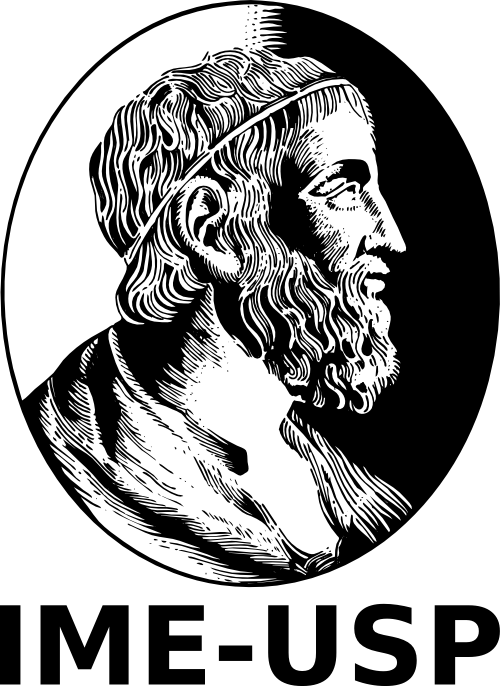
\includegraphics[width=0.25\textwidth]{picstcc/ime.png}
        % \end{figure}}
% \date{2017}


\begin{document}

  \begin{titlepage}
  \begin{center}
   {\huge\bfseries Inteligência Artificial \\ em \textit{Magic: the Gathering}\\}
   % ----------------------------------------------------------------
   \vspace{1.5cm}
   {\bfseries Guilherme Souto Schützer}\\[5pt]
   guischutzer@gmail.com\\[14pt]
   \vspace{0.5cm}
   {\bfseries Tomás Marcondes Bezerra Paim}\\[5pt]
   tomasbmp@gmail.com\\[14pt]
    % ----------------------------------------------------------------
   \vspace{2cm}
  {\begin{figure}[!h]
          \centering
              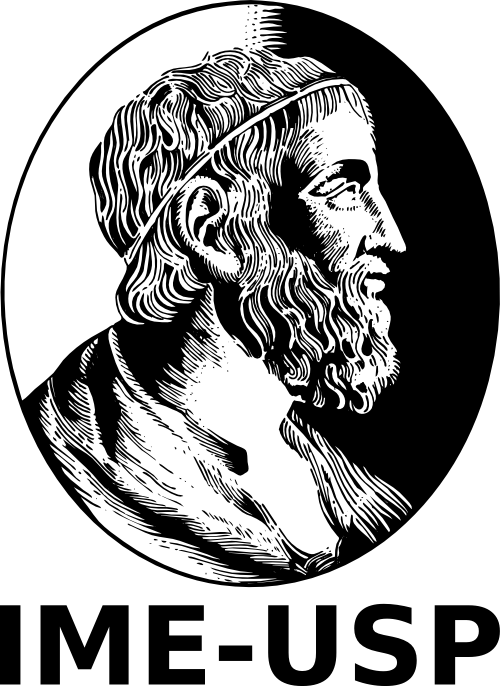
\includegraphics[width=0.25\textwidth]{picstcc/ime.png}
  \end{figure}}
   \vspace{0.4cm}
 \end{center}
  \end{titlepage}

\chapter*{Objetivo}
\textbf{Magic: The Gathering} é um jogo de cartas criado em 1993 por
Richard Garfield que introduziu o conceito moderno de \textit{trading
card game} (jogo de cartas colecionáveis). Com um acervo de mais de 15
mil cartas diferentes, os jogadores devem criar baralhos de 60 cartas
(normalmente podendo haver repetição de até quatro cartas iguais) e
competir, normalmente em jogos um contra um.
\par Durante o jogo, os jogadores têm que lidar com informações
conhecidas (as cartas já jogadas previamente e as cartas em suas mãos) e
informações desconhecidas (as cartas na mão de seu oponente e a ordem
das cartas em seu baralho), o que faz com que seja praticamente
impossível ter informação perfeita. Além disso, ambos os jogadores podem
agir a praticamente qualquer momento dentro de um turno, o que adiciona
uma camada a mais de complexidade.
\par Já existem inteligências artificiais feitas para jogar
\textbf{Magic}, mas devido à complexidade do jogo, nenhuma inteligência
artificial consegue ser realmente boa no jogo (por exemplo, elas não
costumam levar em consideração as cartas que estão na sua mão, então é
muito fácil fazer com que a IA sempre ``morda sua isca'').
\par Nosso objetivo com o trabalho será entender o problema e criar a
nossa versão de uma inteligência artificial para uma versão simplificada
do jogo (limitando o conjunto de cartas disponíveis, adicionando
restrições à construção dos baralhos e simplificando algumas regras do
jogo).

\chapter{Introdução}

\section{Regras básicas}

Um jogo usual de \textit{Magic: the Gathering} conta com dois jogadores
munidos de um baralho de 60 \textit{cards}, ambos começando com 20
pontos de vida, com o objetivo de reduzir o total de pontos de vida do
oponente a 0. Para tanto, é preciso usar os \textit{cards} disponíveis
na mão, que podem representar feitiços, criaturas ou terrenos (existem
outros tipos de \textit{cards}, mas para nossa implementação vamos focar
nesses três). Feitiços são \textit{cards} que têm um efeito que acontece
no momento em que são jogados e então são colocados no cemitério (como é
chamada a pilha de descarte no jogo).\\


Por exemplo, o feitiço Divinação tem um efeito simples: "Compre dois
cards". O jogador que joga este card pega os dois cards do topo de seu
baralho e os coloca em sua mão, aumentando o leque de possibilidades.
Assim, \textbf{feitiços} podem alterar o estado do jogo de diversas
maneiras (como fazer com que os jogadores comprem ou descartem cards,
alterar o total de pontos de vida de um jogador ou destruir uma
criatura) e são a principal forma de interagir com o oponente ou
desenvolver o seu lado do campo de batalha (como é chamada a zona em que
ficam as criaturas e terrenos).

\begin{figure}[!h]
    \centering
    \begin{minipage}{0.45\textwidth}
        \centering
        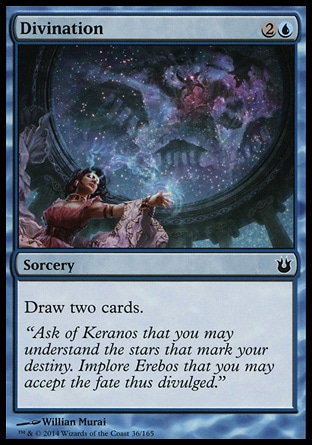
\includegraphics[width=0.5\textwidth]{picstcc/divination.jpg}
        \caption{Divinação (Feitiço)}
        \label{divination}
    \end{minipage}\hfill
    \begin{minipage}{0.45\textwidth}
        \centering
        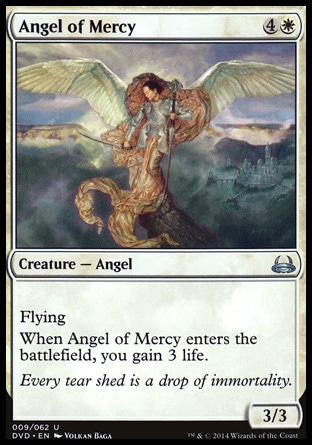
\includegraphics[width=0.5\textwidth]{picstcc/angelOfMercy.jpg}
        \caption{Anjo da Misericórdia (Criatura)}
        \label{anjo}
    \end{minipage}
\end{figure}

\textbf{Criaturas} são cards permanentes (uma vez jogados eles
permanecem no campo de batalha até que sejam destruídos por algum
feitiço ou durante o combate) que possuem poder (quantidade de dano
causado em combate), resistência (quantidade de dano necessária para ser
destruída) e muitas vezes habilidades que afetam o andamento do combate
ou que fazem algum efeito no momento em que são jogadas.

Por exemplo, Anjo da Misericórdia tem a habilidade de Voar (que limita
as interações do oponente durante o combate) e concede a seu controlador
3 pontos de vida ao entrar no campo de batalha. Além disso, seu poder e
resistência são 3 e 3, respectivamente, conforme indicado na caixa no
canto inferior direito.

\textbf{Terrenos} são a fonte de \textit{mana}, que é o recurso
utilizado para pagar por criaturas e feitiços. O custo de \textit{mana}
dos \textit{cards} que não são terreno está indicado no canto superior
direito do card (por exemplo, para jogar Divinação é necessário usar
terrenos, sendo que um deles deve ser necessariamente uma Ilha, como na
\ref{ilha}). Terrenos são, portanto, um dos tipos de \textit{cards}
mais importantes, pois sem eles não há maneira (normalmente) de jogar
seus outros \textit{cards}. A mecânica associada ao uso de recursos é
\textbf{virar} (em inglês, \textit{tap}): para conjurar

\begin{wrapfigure}{R}{5cm}
    \centering
    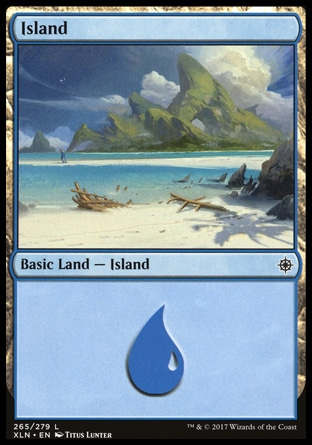
\includegraphics[width=0.25\textwidth]{picstcc/island.jpg}
    \label{ilha}
    \caption{Ilha (Terreno)}
\end{wrapfigure}

Cada ``cor'' de \textit{mana} tem um tipo de terreno associado: assim
como azul (Ilha), temos o branco (Planície), verde (Floresta),
vermelho (Montanha) e preto (Pântano). O jogo inclusive conta com uma
espécie de ``diagrama filosófico'' chamado \textit{Color Pie}
(do inglês, ``torta das cores'', pois se trata de um gráfico circular)
associando cada cor a valores e traços de personalidade.
A título de curiosidade, alguns dos principais aspectos de cada cor são:
conhecimento, para o azul; ordem, em branco; instinto, no verde;
impulso, para o vermelho e amoralidade, característica do preto. Os
aspectos de cada cor são refletidos mecanicamente nas cartas e,
consequentemente, acabam muitas vezes refletindo, em nível mais
abstrato, nas estratégias associadas à montagem e uso dos
\textit{decks}.
Por exemplo: comprar \textit{cards} representa acumular conhecimento,
portanto Divinação é um feitiço que representa bem sua cor.
Entraremos mais a fundo no assunto nas seções futuras, na
apresentação dos decks usados para teste e jogo.

No começo do jogo é decidido aleatoriamente quem será o jogador inicial,
e então os dois jogadores compram uma mão inicial de sete cartas.
Antes do jogo propriamente dito começar, os jogadores tomam as decisões
de \textit{mulligan}, um processo onde cada jogador pode decidir
se aceita a sua mão inicial ou se quer embaralhar de volta suas cartas
no deck e comprar uma nova mão com uma carta a menos, repetir o processo
até que decida manter a mão. Uma vez que os dois jogadores tiverem
escolhido uma mão inicial para manter, cada jogador que realizou pelo
menos um mulligan
olha a carta do topo de seu deck e decide se quer colocá-la no fundo.

O jogo então começa, com os jogadores alternando entre turnos, onde o
jogador que ``controla o turno'' é chamado de \textit{jogador ativo},
com a seguinte estrutura, simplificada (iremos entrar em maiores
detalhes nas próximas seções):

\begin{itemize}
    \item\textbf{Início do turno}: Permanentes do jogador ativo são
desviradas. Jogador ativo compra uma carta de seu \textit{deck}.
    \item\textbf{Primeira Fase Principal}: Jogador ativo pode jogar as
cartas da mão.
    \item \textbf{Combate}: Jogador ativo ``declara atacantes'' (escolhe
quais de suas criaturas irão atacar seu oponente); em seguida, seu
oponente ``declara bloqueadores'' (escolhe quais de suas criaturas irão
bloquear as criaturas atacantes). Cada criatura não-bloqueada, então,
causa dano igual ao seu poder ao oponente e todas as criaturas
bloqueadas e bloqueadoras causam dano entre si.
    \item \textbf{Segunda Fase Principal}: Igual à primeira Fase
Principal.
\end{itemize}

A estrutura acima se repete até o jogo terminar, o que acontece
geralmente quando algum jogador chega a 0 pontos de vida,
mas também pode acontecer de outras maneiras como, por exemplo, se o
baralho de um jogador acabar.

\chapter{Modelagem}

Neste capítulo abordaremos um jogo de \textit{Magic} como um problema de
Inteligência Artificial. A estrutura de um turno, como descrita
 no capítulo anterior, será repetida algumas vezes até o jogo acabar,
porém é necessário determinar a mão inicial de cada jogador e, por isso,
 trataremos este problema em separado.

\section{\textit{Mulligan}}
Baseando-se na experiência própria, a estrutura do problema do
\textbf{\textit{mulligan}} é notavelmente diferente do resto de um jogo
de \textit{Magic}.
A principal diferença é que apesar de ambos os jogadores tomarem
decisões alternadamente nessa etapa, as ações do oponente não têm
nenhuma influência
direta sobre as ações do agente, que deve se concentrar em obter uma
\textbf{mão inicial} que possibilite jogadas nos primeiros turnos do
jogo.
A figura \ref{mulligan} representa as escolhas que o jogador poderá
fazer para determiná-la, com cada conjunto de cartas representando um
conjunto
de estados.

\begin{figure}
  \centering
  \label{mulligan}
  % Graphic for TeX using PGF
% Title: /home/schutzer/comp/mtcc_super/mtcc_support/mulligan.dia
% Creator: Dia v0.97.3
% CreationDate: Fri Nov 10 11:39:18 2017
% For: schutzer
% \usepackage{tikz}
% The following commands are not supported in PSTricks at present
% We define them conditionally, so when they are implemented,
% this pgf file will use them.
\ifx\du\undefined
  \newlength{\du}
\fi
\setlength{\du}{15\unitlength}
\begin{tikzpicture}[scale=0.35]
\pgftransformxscale{1.000000}
\pgftransformyscale{-1.000000}
\definecolor{dialinecolor}{rgb}{0.000000, 0.000000, 0.000000}
\pgfsetstrokecolor{dialinecolor}
\definecolor{dialinecolor}{rgb}{1.000000, 1.000000, 1.000000}
\pgfsetfillcolor{dialinecolor}
\pgfsetlinewidth{0.100000\du}
\pgfsetdash{}{0pt}
\pgfsetdash{}{0pt}
\pgfsetmiterjoin
\definecolor{dialinecolor}{rgb}{1.000000, 1.000000, 1.000000}
\pgfsetfillcolor{dialinecolor}
\fill (31.000000\du,12.231300\du)--(31.000000\du,19.231300\du)--(36.000000\du,19.231300\du)--(36.000000\du,12.231300\du)--cycle;
\definecolor{dialinecolor}{rgb}{0.000000, 0.000000, 0.000000}
\pgfsetstrokecolor{dialinecolor}
\draw (31.000000\du,12.231300\du)--(31.000000\du,19.231300\du)--(36.000000\du,19.231300\du)--(36.000000\du,12.231300\du)--cycle;
\pgfsetlinewidth{0.100000\du}
\pgfsetdash{}{0pt}
\pgfsetdash{}{0pt}
\pgfsetmiterjoin
\definecolor{dialinecolor}{rgb}{1.000000, 1.000000, 1.000000}
\pgfsetfillcolor{dialinecolor}
\fill (30.000000\du,11.231300\du)--(30.000000\du,18.231300\du)--(35.000000\du,18.231300\du)--(35.000000\du,11.231300\du)--cycle;
\definecolor{dialinecolor}{rgb}{0.000000, 0.000000, 0.000000}
\pgfsetstrokecolor{dialinecolor}
\draw (30.000000\du,11.231300\du)--(30.000000\du,18.231300\du)--(35.000000\du,18.231300\du)--(35.000000\du,11.231300\du)--cycle;
\pgfsetlinewidth{0.100000\du}
\pgfsetdash{}{0pt}
\pgfsetdash{}{0pt}
\pgfsetmiterjoin
\definecolor{dialinecolor}{rgb}{1.000000, 1.000000, 1.000000}
\pgfsetfillcolor{dialinecolor}
\fill (29.000000\du,10.231300\du)--(29.000000\du,17.231300\du)--(34.000000\du,17.231300\du)--(34.000000\du,10.231300\du)--cycle;
\definecolor{dialinecolor}{rgb}{0.000000, 0.000000, 0.000000}
\pgfsetstrokecolor{dialinecolor}
\draw (29.000000\du,10.231300\du)--(29.000000\du,17.231300\du)--(34.000000\du,17.231300\du)--(34.000000\du,10.231300\du)--cycle;
\pgfsetlinewidth{0.100000\du}
\pgfsetdash{}{0pt}
\pgfsetdash{}{0pt}
\pgfsetmiterjoin
\definecolor{dialinecolor}{rgb}{1.000000, 1.000000, 1.000000}
\pgfsetfillcolor{dialinecolor}
\fill (28.000000\du,9.231330\du)--(28.000000\du,16.231330\du)--(33.000000\du,16.231330\du)--(33.000000\du,9.231330\du)--cycle;
\definecolor{dialinecolor}{rgb}{0.000000, 0.000000, 0.000000}
\pgfsetstrokecolor{dialinecolor}
\draw (28.000000\du,9.231330\du)--(28.000000\du,16.231330\du)--(33.000000\du,16.231330\du)--(33.000000\du,9.231330\du)--cycle;
\pgfsetlinewidth{0.100000\du}
\pgfsetdash{}{0pt}
\pgfsetdash{}{0pt}
\pgfsetmiterjoin
\definecolor{dialinecolor}{rgb}{1.000000, 1.000000, 1.000000}
\pgfsetfillcolor{dialinecolor}
\fill (27.000000\du,8.231330\du)--(27.000000\du,15.231330\du)--(32.000000\du,15.231330\du)--(32.000000\du,8.231330\du)--cycle;
\definecolor{dialinecolor}{rgb}{0.000000, 0.000000, 0.000000}
\pgfsetstrokecolor{dialinecolor}
\draw (27.000000\du,8.231330\du)--(27.000000\du,15.231330\du)--(32.000000\du,15.231330\du)--(32.000000\du,8.231330\du)--cycle;
\pgfsetlinewidth{0.100000\du}
\pgfsetdash{}{0pt}
\pgfsetdash{}{0pt}
\pgfsetmiterjoin
\definecolor{dialinecolor}{rgb}{1.000000, 1.000000, 1.000000}
\pgfsetfillcolor{dialinecolor}
\fill (26.000000\du,7.231330\du)--(26.000000\du,14.231330\du)--(31.000000\du,14.231330\du)--(31.000000\du,7.231330\du)--cycle;
\definecolor{dialinecolor}{rgb}{0.000000, 0.000000, 0.000000}
\pgfsetstrokecolor{dialinecolor}
\draw (26.000000\du,7.231330\du)--(26.000000\du,14.231330\du)--(31.000000\du,14.231330\du)--(31.000000\du,7.231330\du)--cycle;
\pgfsetlinewidth{0.100000\du}
\pgfsetdash{}{0pt}
\pgfsetdash{}{0pt}
\pgfsetmiterjoin
\definecolor{dialinecolor}{rgb}{1.000000, 1.000000, 1.000000}
\pgfsetfillcolor{dialinecolor}
\fill (25.000000\du,6.231330\du)--(25.000000\du,13.231330\du)--(30.000000\du,13.231330\du)--(30.000000\du,6.231330\du)--cycle;
\definecolor{dialinecolor}{rgb}{0.000000, 0.000000, 0.000000}
\pgfsetstrokecolor{dialinecolor}
\draw (25.000000\du,6.231330\du)--(25.000000\du,13.231330\du)--(30.000000\du,13.231330\du)--(30.000000\du,6.231330\du)--cycle;
\pgfsetlinewidth{0.100000\du}
\pgfsetdash{}{0pt}
\pgfsetdash{}{0pt}
\pgfsetmiterjoin
\definecolor{dialinecolor}{rgb}{1.000000, 1.000000, 1.000000}
\pgfsetfillcolor{dialinecolor}
\fill (36.000000\du,29.000000\du)--(36.000000\du,36.000000\du)--(41.000000\du,36.000000\du)--(41.000000\du,29.000000\du)--cycle;
\definecolor{dialinecolor}{rgb}{0.000000, 0.000000, 0.000000}
\pgfsetstrokecolor{dialinecolor}
\draw (36.000000\du,29.000000\du)--(36.000000\du,36.000000\du)--(41.000000\du,36.000000\du)--(41.000000\du,29.000000\du)--cycle;
\pgfsetlinewidth{0.100000\du}
\pgfsetdash{}{0pt}
\pgfsetdash{}{0pt}
\pgfsetmiterjoin
\definecolor{dialinecolor}{rgb}{1.000000, 1.000000, 1.000000}
\pgfsetfillcolor{dialinecolor}
\fill (35.000000\du,28.000000\du)--(35.000000\du,35.000000\du)--(40.000000\du,35.000000\du)--(40.000000\du,28.000000\du)--cycle;
\definecolor{dialinecolor}{rgb}{0.000000, 0.000000, 0.000000}
\pgfsetstrokecolor{dialinecolor}
\draw (35.000000\du,28.000000\du)--(35.000000\du,35.000000\du)--(40.000000\du,35.000000\du)--(40.000000\du,28.000000\du)--cycle;
\pgfsetlinewidth{0.100000\du}
\pgfsetdash{}{0pt}
\pgfsetdash{}{0pt}
\pgfsetmiterjoin
\definecolor{dialinecolor}{rgb}{1.000000, 1.000000, 1.000000}
\pgfsetfillcolor{dialinecolor}
\fill (34.000000\du,27.000000\du)--(34.000000\du,34.000000\du)--(39.000000\du,34.000000\du)--(39.000000\du,27.000000\du)--cycle;
\definecolor{dialinecolor}{rgb}{0.000000, 0.000000, 0.000000}
\pgfsetstrokecolor{dialinecolor}
\draw (34.000000\du,27.000000\du)--(34.000000\du,34.000000\du)--(39.000000\du,34.000000\du)--(39.000000\du,27.000000\du)--cycle;
\pgfsetlinewidth{0.100000\du}
\pgfsetdash{}{0pt}
\pgfsetdash{}{0pt}
\pgfsetmiterjoin
\definecolor{dialinecolor}{rgb}{1.000000, 1.000000, 1.000000}
\pgfsetfillcolor{dialinecolor}
\fill (33.000000\du,26.000000\du)--(33.000000\du,33.000000\du)--(38.000000\du,33.000000\du)--(38.000000\du,26.000000\du)--cycle;
\definecolor{dialinecolor}{rgb}{0.000000, 0.000000, 0.000000}
\pgfsetstrokecolor{dialinecolor}
\draw (33.000000\du,26.000000\du)--(33.000000\du,33.000000\du)--(38.000000\du,33.000000\du)--(38.000000\du,26.000000\du)--cycle;
\pgfsetlinewidth{0.100000\du}
\pgfsetdash{}{0pt}
\pgfsetdash{}{0pt}
\pgfsetmiterjoin
\definecolor{dialinecolor}{rgb}{1.000000, 1.000000, 1.000000}
\pgfsetfillcolor{dialinecolor}
\fill (32.000000\du,25.000000\du)--(32.000000\du,32.000000\du)--(37.000000\du,32.000000\du)--(37.000000\du,25.000000\du)--cycle;
\definecolor{dialinecolor}{rgb}{0.000000, 0.000000, 0.000000}
\pgfsetstrokecolor{dialinecolor}
\draw (32.000000\du,25.000000\du)--(32.000000\du,32.000000\du)--(37.000000\du,32.000000\du)--(37.000000\du,25.000000\du)--cycle;
\pgfsetlinewidth{0.100000\du}
\pgfsetdash{}{0pt}
\pgfsetdash{}{0pt}
\pgfsetmiterjoin
\definecolor{dialinecolor}{rgb}{1.000000, 1.000000, 1.000000}
\pgfsetfillcolor{dialinecolor}
\fill (31.000000\du,24.000000\du)--(31.000000\du,31.000000\du)--(36.000000\du,31.000000\du)--(36.000000\du,24.000000\du)--cycle;
\definecolor{dialinecolor}{rgb}{0.000000, 0.000000, 0.000000}
\pgfsetstrokecolor{dialinecolor}
\draw (31.000000\du,24.000000\du)--(31.000000\du,31.000000\du)--(36.000000\du,31.000000\du)--(36.000000\du,24.000000\du)--cycle;
\definecolor{dialinecolor}{rgb}{1.000000, 1.000000, 1.000000}
\pgfsetfillcolor{dialinecolor}
\fill (54.005330\du,14.000000\du)--(56.010660\du,15.752665\du)--(54.005330\du,17.505330\du)--(52.000000\du,15.752665\du)--cycle;
\pgfsetlinewidth{0.100000\du}
\pgfsetdash{}{0pt}
\pgfsetdash{}{0pt}
\pgfsetmiterjoin
\definecolor{dialinecolor}{rgb}{0.000000, 0.000000, 0.000000}
\pgfsetstrokecolor{dialinecolor}
\draw (54.005330\du,14.000000\du)--(56.010660\du,15.752665\du)--(54.005330\du,17.505330\du)--(52.000000\du,15.752665\du)--cycle;
% setfont left to latex
\definecolor{dialinecolor}{rgb}{0.000000, 0.000000, 0.000000}
\pgfsetstrokecolor{dialinecolor}
\node at (54.005330\du,15.947665\du){};
\pgfsetlinewidth{0.100000\du}
\pgfsetdash{}{0pt}
\pgfsetdash{}{0pt}
\pgfsetbuttcap
{
\definecolor{dialinecolor}{rgb}{0.000000, 0.000000, 0.000000}
\pgfsetfillcolor{dialinecolor}
% was here!!!
\pgfsetarrowsend{stealth}
\definecolor{dialinecolor}{rgb}{0.000000, 0.000000, 0.000000}
\pgfsetstrokecolor{dialinecolor}
\draw (36.049399\du,15.733956\du)--(51.950000\du,15.750524\du);
}
\definecolor{dialinecolor}{rgb}{1.000000, 1.000000, 1.000000}
\pgfsetfillcolor{dialinecolor}
\pgfpathellipse{\pgfpoint{70.343600\du}{15.752300\du}}{\pgfpoint{2.500000\du}{0\du}}{\pgfpoint{0\du}{2.500000\du}}
\pgfusepath{fill}
\pgfsetlinewidth{0.100000\du}
\pgfsetdash{}{0pt}
\pgfsetdash{}{0pt}
\pgfsetmiterjoin
\definecolor{dialinecolor}{rgb}{0.000000, 0.000000, 0.000000}
\pgfsetstrokecolor{dialinecolor}
\pgfpathellipse{\pgfpoint{70.343600\du}{15.752300\du}}{\pgfpoint{2.500000\du}{0\du}}{\pgfpoint{0\du}{2.500000\du}}
\pgfusepath{stroke}
% setfont left to latex
\definecolor{dialinecolor}{rgb}{0.000000, 0.000000, 0.000000}
\pgfsetstrokecolor{dialinecolor}
\node at (70.343600\du,15.947300\du){};
\definecolor{dialinecolor}{rgb}{1.000000, 1.000000, 1.000000}
\pgfsetfillcolor{dialinecolor}
\fill (54.005330\du,30.691600\du)--(56.010660\du,32.444265\du)--(54.005330\du,34.196930\du)--(52.000000\du,32.444265\du)--cycle;
\pgfsetlinewidth{0.100000\du}
\pgfsetdash{}{0pt}
\pgfsetdash{}{0pt}
\pgfsetmiterjoin
\definecolor{dialinecolor}{rgb}{0.000000, 0.000000, 0.000000}
\pgfsetstrokecolor{dialinecolor}
\draw (54.005330\du,30.691600\du)--(56.010660\du,32.444265\du)--(54.005330\du,34.196930\du)--(52.000000\du,32.444265\du)--cycle;
% setfont left to latex
\definecolor{dialinecolor}{rgb}{0.000000, 0.000000, 0.000000}
\pgfsetstrokecolor{dialinecolor}
\node at (54.005330\du,32.639265\du){};
\pgfsetlinewidth{0.100000\du}
\pgfsetdash{}{0pt}
\pgfsetdash{}{0pt}
\pgfsetmiterjoin
\definecolor{dialinecolor}{rgb}{1.000000, 1.000000, 1.000000}
\pgfsetfillcolor{dialinecolor}
\fill (40.000000\du,44.000000\du)--(40.000000\du,51.000000\du)--(45.000000\du,51.000000\du)--(45.000000\du,44.000000\du)--cycle;
\definecolor{dialinecolor}{rgb}{0.000000, 0.000000, 0.000000}
\pgfsetstrokecolor{dialinecolor}
\draw (40.000000\du,44.000000\du)--(40.000000\du,51.000000\du)--(45.000000\du,51.000000\du)--(45.000000\du,44.000000\du)--cycle;
\pgfsetlinewidth{0.100000\du}
\pgfsetdash{}{0pt}
\pgfsetdash{}{0pt}
\pgfsetmiterjoin
\definecolor{dialinecolor}{rgb}{1.000000, 1.000000, 1.000000}
\pgfsetfillcolor{dialinecolor}
\fill (39.000000\du,43.000000\du)--(39.000000\du,50.000000\du)--(44.000000\du,50.000000\du)--(44.000000\du,43.000000\du)--cycle;
\definecolor{dialinecolor}{rgb}{0.000000, 0.000000, 0.000000}
\pgfsetstrokecolor{dialinecolor}
\draw (39.000000\du,43.000000\du)--(39.000000\du,50.000000\du)--(44.000000\du,50.000000\du)--(44.000000\du,43.000000\du)--cycle;
\pgfsetlinewidth{0.100000\du}
\pgfsetdash{}{0pt}
\pgfsetdash{}{0pt}
\pgfsetmiterjoin
\definecolor{dialinecolor}{rgb}{1.000000, 1.000000, 1.000000}
\pgfsetfillcolor{dialinecolor}
\fill (38.000000\du,42.000000\du)--(38.000000\du,49.000000\du)--(43.000000\du,49.000000\du)--(43.000000\du,42.000000\du)--cycle;
\definecolor{dialinecolor}{rgb}{0.000000, 0.000000, 0.000000}
\pgfsetstrokecolor{dialinecolor}
\draw (38.000000\du,42.000000\du)--(38.000000\du,49.000000\du)--(43.000000\du,49.000000\du)--(43.000000\du,42.000000\du)--cycle;
\pgfsetlinewidth{0.100000\du}
\pgfsetdash{}{0pt}
\pgfsetdash{}{0pt}
\pgfsetmiterjoin
\definecolor{dialinecolor}{rgb}{1.000000, 1.000000, 1.000000}
\pgfsetfillcolor{dialinecolor}
\fill (37.000000\du,41.000000\du)--(37.000000\du,48.000000\du)--(42.000000\du,48.000000\du)--(42.000000\du,41.000000\du)--cycle;
\definecolor{dialinecolor}{rgb}{0.000000, 0.000000, 0.000000}
\pgfsetstrokecolor{dialinecolor}
\draw (37.000000\du,41.000000\du)--(37.000000\du,48.000000\du)--(42.000000\du,48.000000\du)--(42.000000\du,41.000000\du)--cycle;
\pgfsetlinewidth{0.100000\du}
\pgfsetdash{}{0pt}
\pgfsetdash{}{0pt}
\pgfsetmiterjoin
\definecolor{dialinecolor}{rgb}{1.000000, 1.000000, 1.000000}
\pgfsetfillcolor{dialinecolor}
\fill (36.000000\du,40.000000\du)--(36.000000\du,47.000000\du)--(41.000000\du,47.000000\du)--(41.000000\du,40.000000\du)--cycle;
\definecolor{dialinecolor}{rgb}{0.000000, 0.000000, 0.000000}
\pgfsetstrokecolor{dialinecolor}
\draw (36.000000\du,40.000000\du)--(36.000000\du,47.000000\du)--(41.000000\du,47.000000\du)--(41.000000\du,40.000000\du)--cycle;
\pgfsetlinewidth{0.100000\du}
\pgfsetdash{}{0pt}
\pgfsetdash{}{0pt}
\pgfsetmiterjoin
\definecolor{dialinecolor}{rgb}{1.000000, 1.000000, 1.000000}
\pgfsetfillcolor{dialinecolor}
\fill (40.000000\du,68.000000\du)--(40.000000\du,75.000000\du)--(45.000000\du,75.000000\du)--(45.000000\du,68.000000\du)--cycle;
\definecolor{dialinecolor}{rgb}{0.000000, 0.000000, 0.000000}
\pgfsetstrokecolor{dialinecolor}
\draw (40.000000\du,68.000000\du)--(40.000000\du,75.000000\du)--(45.000000\du,75.000000\du)--(45.000000\du,68.000000\du)--cycle;
% setfont left to latex
\definecolor{dialinecolor}{rgb}{0.000000, 0.000000, 0.000000}
\pgfsetstrokecolor{dialinecolor}
\node[anchor=west] at (59.500000\du,14.300000\du){$K$};
\pgfsetlinewidth{0.100000\du}
\pgfsetdash{}{0pt}
\pgfsetdash{}{0pt}
\pgfsetbuttcap
{
\definecolor{dialinecolor}{rgb}{0.000000, 0.000000, 0.000000}
\pgfsetfillcolor{dialinecolor}
% was here!!!
\pgfsetarrowsend{stealth}
\definecolor{dialinecolor}{rgb}{0.000000, 0.000000, 0.000000}
\pgfsetstrokecolor{dialinecolor}
\draw (41.049789\du,32.489480\du)--(52.000000\du,32.444300\du);
}
\definecolor{dialinecolor}{rgb}{1.000000, 1.000000, 1.000000}
\pgfsetfillcolor{dialinecolor}
\fill (54.005330\du,45.793300\du)--(56.010660\du,47.545965\du)--(54.005330\du,49.298630\du)--(52.000000\du,47.545965\du)--cycle;
\pgfsetlinewidth{0.100000\du}
\pgfsetdash{}{0pt}
\pgfsetdash{}{0pt}
\pgfsetmiterjoin
\definecolor{dialinecolor}{rgb}{0.000000, 0.000000, 0.000000}
\pgfsetstrokecolor{dialinecolor}
\draw (54.005330\du,45.793300\du)--(56.010660\du,47.545965\du)--(54.005330\du,49.298630\du)--(52.000000\du,47.545965\du)--cycle;
% setfont left to latex
\definecolor{dialinecolor}{rgb}{0.000000, 0.000000, 0.000000}
\pgfsetstrokecolor{dialinecolor}
\node at (54.005330\du,47.740965\du){};
% setfont left to latex
\definecolor{dialinecolor}{rgb}{0.000000, 0.000000, 0.000000}
\pgfsetstrokecolor{dialinecolor}
\node[anchor=west] at (69.000000\du,68.116600\du){};
% setfont left to latex
\definecolor{dialinecolor}{rgb}{0.000000, 0.000000, 0.000000}
\pgfsetstrokecolor{dialinecolor}
\node[anchor=west] at (69.000000\du,46.294500\du){};
\definecolor{dialinecolor}{rgb}{1.000000, 1.000000, 1.000000}
\pgfsetfillcolor{dialinecolor}
\fill (70.174430\du,44.500000\du)--(73.348860\du,47.603350\du)--(70.174430\du,50.706700\du)--(67.000000\du,47.603350\du)--cycle;
\pgfsetlinewidth{0.100000\du}
\pgfsetdash{}{0pt}
\pgfsetdash{}{0pt}
\pgfsetmiterjoin
\definecolor{dialinecolor}{rgb}{0.000000, 0.000000, 0.000000}
\pgfsetstrokecolor{dialinecolor}
\draw (70.174430\du,44.500000\du)--(73.348860\du,47.603350\du)--(70.174430\du,50.706700\du)--(67.000000\du,47.603350\du)--cycle;
% setfont left to latex
\definecolor{dialinecolor}{rgb}{0.000000, 0.000000, 0.000000}
\pgfsetstrokecolor{dialinecolor}
\node at (70.174430\du,47.798350\du){$scry$};
\definecolor{dialinecolor}{rgb}{1.000000, 1.000000, 1.000000}
\pgfsetfillcolor{dialinecolor}
\pgfpathellipse{\pgfpoint{65.558300\du}{56.535900\du}}{\pgfpoint{2.500000\du}{0\du}}{\pgfpoint{0\du}{2.500000\du}}
\pgfusepath{fill}
\pgfsetlinewidth{0.100000\du}
\pgfsetdash{}{0pt}
\pgfsetdash{}{0pt}
\pgfsetmiterjoin
\definecolor{dialinecolor}{rgb}{0.000000, 0.000000, 0.000000}
\pgfsetstrokecolor{dialinecolor}
\pgfpathellipse{\pgfpoint{65.558300\du}{56.535900\du}}{\pgfpoint{2.500000\du}{0\du}}{\pgfpoint{0\du}{2.500000\du}}
\pgfusepath{stroke}
% setfont left to latex
\definecolor{dialinecolor}{rgb}{0.000000, 0.000000, 0.000000}
\pgfsetstrokecolor{dialinecolor}
\node at (65.558300\du,56.730900\du){};
\definecolor{dialinecolor}{rgb}{1.000000, 1.000000, 1.000000}
\pgfsetfillcolor{dialinecolor}
\pgfpathellipse{\pgfpoint{75.549200\du}{56.535900\du}}{\pgfpoint{2.500000\du}{0\du}}{\pgfpoint{0\du}{2.500000\du}}
\pgfusepath{fill}
\pgfsetlinewidth{0.100000\du}
\pgfsetdash{}{0pt}
\pgfsetdash{}{0pt}
\pgfsetmiterjoin
\definecolor{dialinecolor}{rgb}{0.000000, 0.000000, 0.000000}
\pgfsetstrokecolor{dialinecolor}
\pgfpathellipse{\pgfpoint{75.549200\du}{56.535900\du}}{\pgfpoint{2.500000\du}{0\du}}{\pgfpoint{0\du}{2.500000\du}}
\pgfusepath{stroke}
% setfont left to latex
\definecolor{dialinecolor}{rgb}{0.000000, 0.000000, 0.000000}
\pgfsetstrokecolor{dialinecolor}
\node at (75.549200\du,56.730900\du){};
\pgfsetlinewidth{0.100000\du}
\pgfsetdash{}{0pt}
\pgfsetdash{}{0pt}
\pgfsetbuttcap
{
\definecolor{dialinecolor}{rgb}{0.000000, 0.000000, 0.000000}
\pgfsetfillcolor{dialinecolor}
% was here!!!
\pgfsetarrowsend{stealth}
\definecolor{dialinecolor}{rgb}{0.000000, 0.000000, 0.000000}
\pgfsetstrokecolor{dialinecolor}
\draw (69.091820\du,49.698279\du)--(66.728674\du,54.271141\du);
}
\pgfsetlinewidth{0.100000\du}
\pgfsetdash{}{0pt}
\pgfsetdash{}{0pt}
\pgfsetbuttcap
{
\definecolor{dialinecolor}{rgb}{0.000000, 0.000000, 0.000000}
\pgfsetfillcolor{dialinecolor}
% was here!!!
\pgfsetarrowsend{stealth}
\definecolor{dialinecolor}{rgb}{0.000000, 0.000000, 0.000000}
\pgfsetstrokecolor{dialinecolor}
\draw (71.368860\du,49.588422\du)--(74.235688\du,54.352921\du);
}
\pgfsetlinewidth{0.100000\du}
\pgfsetdash{}{0pt}
\pgfsetdash{}{0pt}
\pgfsetbuttcap
{
\definecolor{dialinecolor}{rgb}{0.000000, 0.000000, 0.000000}
\pgfsetfillcolor{dialinecolor}
% was here!!!
\pgfsetarrowsend{stealth}
\definecolor{dialinecolor}{rgb}{0.000000, 0.000000, 0.000000}
\pgfsetstrokecolor{dialinecolor}
\draw (56.056369\du,47.555023\du)--(67.000000\du,47.603350\du);
}
\pgfsetlinewidth{0.100000\du}
\pgfsetdash{}{0pt}
\pgfsetdash{}{0pt}
\pgfsetbuttcap
{
\definecolor{dialinecolor}{rgb}{0.000000, 0.000000, 0.000000}
\pgfsetfillcolor{dialinecolor}
% was here!!!
\pgfsetarrowsend{stealth}
\definecolor{dialinecolor}{rgb}{0.000000, 0.000000, 0.000000}
\pgfsetstrokecolor{dialinecolor}
\draw (45.000000\du,47.500000\du)--(52.000000\du,47.546000\du);
}
\definecolor{dialinecolor}{rgb}{1.000000, 1.000000, 1.000000}
\pgfsetfillcolor{dialinecolor}
\fill (54.005330\du,69.762200\du)--(56.010660\du,71.514865\du)--(54.005330\du,73.267530\du)--(52.000000\du,71.514865\du)--cycle;
\pgfsetlinewidth{0.100000\du}
\pgfsetdash{}{0pt}
\pgfsetdash{}{0pt}
\pgfsetmiterjoin
\definecolor{dialinecolor}{rgb}{0.000000, 0.000000, 0.000000}
\pgfsetstrokecolor{dialinecolor}
\draw (54.005330\du,69.762200\du)--(56.010660\du,71.514865\du)--(54.005330\du,73.267530\du)--(52.000000\du,71.514865\du)--cycle;
% setfont left to latex
\definecolor{dialinecolor}{rgb}{0.000000, 0.000000, 0.000000}
\pgfsetstrokecolor{dialinecolor}
\node at (54.005330\du,71.709865\du){};
\pgfsetlinewidth{0.100000\du}
\pgfsetdash{}{0pt}
\pgfsetdash{}{0pt}
\pgfsetbuttcap
{
\definecolor{dialinecolor}{rgb}{0.000000, 0.000000, 0.000000}
\pgfsetfillcolor{dialinecolor}
% was here!!!
\pgfsetarrowsend{stealth}
\definecolor{dialinecolor}{rgb}{0.000000, 0.000000, 0.000000}
\pgfsetstrokecolor{dialinecolor}
\draw (45.049530\du,71.503999\du)--(52.000000\du,71.514900\du);
}
% setfont left to latex
\definecolor{dialinecolor}{rgb}{0.000000, 0.000000, 0.000000}
\pgfsetstrokecolor{dialinecolor}
\node[anchor=east] at (18.000000\du,15.917000\du){$h=7$};
% setfont left to latex
\definecolor{dialinecolor}{rgb}{0.000000, 0.000000, 0.000000}
\pgfsetstrokecolor{dialinecolor}
\node[anchor=east] at (18.000000\du,32.275100\du){6};
% setfont left to latex
\definecolor{dialinecolor}{rgb}{0.000000, 0.000000, 0.000000}
\pgfsetstrokecolor{dialinecolor}
\node[anchor=east] at (18.000000\du,48.000000\du){5};
% setfont left to latex
\definecolor{dialinecolor}{rgb}{0.000000, 0.000000, 0.000000}
\pgfsetstrokecolor{dialinecolor}
\node[anchor=east] at (18.000000\du,72.000000\du){1};
% setfont left to latex
\definecolor{dialinecolor}{rgb}{0.000000, 0.000000, 0.000000}
\pgfsetstrokecolor{dialinecolor}
\node[anchor=east] at (18.000000\du,85.000000\du){0};

\pgfsetlinewidth{0.100000\du}
\pgfsetbuttcap
{
\definecolor{dialinecolor}{rgb}{0.000000, 0.000000, 0.000000}
\pgfsetfillcolor{dialinecolor}
% was here!!!
\pgfsetarrowsend{stealth}
\definecolor{dialinecolor}{rgb}{0.000000, 0.000000, 0.000000}
\pgfsetstrokecolor{dialinecolor}
\draw (56.060660\du,15.752611\du)--(67.843600\du,15.752300\du);
}
% setfont left to latex
\definecolor{dialinecolor}{rgb}{0.000000, 0.000000, 0.000000}
\pgfsetstrokecolor{dialinecolor}
\node[anchor=west] at (59.500000\du,31.000000\du){$K$};
% setfont left to latex
\definecolor{dialinecolor}{rgb}{0.000000, 0.000000, 0.000000}
\pgfsetstrokecolor{dialinecolor}
\node[anchor=west] at (59.500000\du,46.200000\du){$K$};
% setfont left to latex
\definecolor{dialinecolor}{rgb}{0.000000, 0.000000, 0.000000}
\pgfsetstrokecolor{dialinecolor}
\node[anchor=west] at (59.500000\du,70.000000\du){$K$};

\pgfsetlinewidth{0.100000\du}
\pgfsetdash{}{0pt}
\pgfsetdash{}{0pt}
\pgfsetbuttcap
{
\definecolor{dialinecolor}{rgb}{0.000000, 0.000000, 0.000000}
\pgfsetfillcolor{dialinecolor}
% was here!!!
\pgfsetarrowsend{stealth}
\definecolor{dialinecolor}{rgb}{0.000000, 0.000000, 0.000000}
\pgfsetstrokecolor{dialinecolor}
\draw (53.002700\du,16.629000\du)--(33.500000\du,24.000000\du);
}
\pgfsetlinewidth{0.100000\du}
\pgfsetdash{}{0pt}
\pgfsetdash{}{0pt}
\pgfsetbuttcap
{
\definecolor{dialinecolor}{rgb}{0.000000, 0.000000, 0.000000}
\pgfsetfillcolor{dialinecolor}
% was here!!!
\pgfsetarrowsend{stealth}
\definecolor{dialinecolor}{rgb}{0.000000, 0.000000, 0.000000}
\pgfsetstrokecolor{dialinecolor}
\draw (53.002700\du,33.320600\du)--(38.500000\du,40.000000\du);
}
\pgfsetlinewidth{0.100000\du}
\pgfsetdash{{1.000000\du}{1.000000\du}}{0\du}
\pgfsetdash{{1.000000\du}{1.000000\du}}{0\du}
\pgfsetbuttcap
{
\definecolor{dialinecolor}{rgb}{0.000000, 0.000000, 0.000000}
\pgfsetfillcolor{dialinecolor}
% was here!!!
\pgfsetarrowsend{stealth}
\definecolor{dialinecolor}{rgb}{0.000000, 0.000000, 0.000000}
\pgfsetstrokecolor{dialinecolor}
\draw (53.002700\du,48.422300\du)--(42.500000\du,68.000000\du);
}
\definecolor{dialinecolor}{rgb}{0.000000, 0.000000, 0.000000}
\pgfsetstrokecolor{dialinecolor}
\draw (52.529966\du,49.303505\du)--(42.500000\du,68.000000\du);
\pgfsetlinewidth{0.100000\du}
\pgfsetdash{}{0pt}
\definecolor{dialinecolor}{rgb}{0.000000, 0.000000, 0.000000}
\pgfsetstrokecolor{dialinecolor}
\draw (53.002700\du,48.422300\du)--(52.908153\du,48.598541\du);
\definecolor{dialinecolor}{rgb}{0.000000, 0.000000, 0.000000}
\pgfsetstrokecolor{dialinecolor}
\draw (52.845122\du,48.716035\du)--(52.750575\du,48.892276\du);
\definecolor{dialinecolor}{rgb}{0.000000, 0.000000, 0.000000}
\pgfsetstrokecolor{dialinecolor}
\draw (52.687544\du,49.009770\du)--(52.592998\du,49.186011\du);
% setfont left to latex
\definecolor{dialinecolor}{rgb}{0.000000, 0.000000, 0.000000}
\pgfsetstrokecolor{dialinecolor}
\node[anchor=west] at (43.000000\du,22.000000\du){$M$};
% setfont left to latex
\definecolor{dialinecolor}{rgb}{0.000000, 0.000000, 0.000000}
\pgfsetstrokecolor{dialinecolor}
\node[anchor=west] at (48.000000\du,59.000000\du){$M$};
% setfont left to latex
\definecolor{dialinecolor}{rgb}{0.000000, 0.000000, 0.000000}
\pgfsetstrokecolor{dialinecolor}
\node[anchor=west] at (46.000000\du,38.400000\du){$M$};
% setfont left to latex
\definecolor{dialinecolor}{rgb}{0.000000, 0.000000, 0.000000}
\pgfsetstrokecolor{dialinecolor}
\node[anchor=west] at (48.000000\du,78.000000\du){$M$};
% setfont left to latex
\definecolor{dialinecolor}{rgb}{0.000000, 0.000000, 0.000000}
\pgfsetstrokecolor{dialinecolor}
\node[anchor=west] at (70.174430\du,47.603350\du){};
% setfont left to latex
\definecolor{dialinecolor}{rgb}{0.000000, 0.000000, 0.000000}
\pgfsetstrokecolor{dialinecolor}
\node[anchor=west] at (70.343530\du,31.517665\du){};
\definecolor{dialinecolor}{rgb}{1.000000, 1.000000, 1.000000}
\pgfsetfillcolor{dialinecolor}
\fill (70.116130\du,29.264100\du)--(73.290560\du,32.367450\du)--(70.116130\du,35.470800\du)--(66.941700\du,32.367450\du)--cycle;
\pgfsetlinewidth{0.100000\du}
\pgfsetdash{}{0pt}
\pgfsetdash{}{0pt}
\pgfsetmiterjoin
\definecolor{dialinecolor}{rgb}{0.000000, 0.000000, 0.000000}
\pgfsetstrokecolor{dialinecolor}
\draw (70.116130\du,29.264100\du)--(73.290560\du,32.367450\du)--(70.116130\du,35.470800\du)--(66.941700\du,32.367450\du)--cycle;
% setfont left to latex
\definecolor{dialinecolor}{rgb}{0.000000, 0.000000, 0.000000}
\pgfsetstrokecolor{dialinecolor}
\node at (70.116130\du,32.562450\du){$scry$};
\definecolor{dialinecolor}{rgb}{1.000000, 1.000000, 1.000000}
\pgfsetfillcolor{dialinecolor}
\pgfpathellipse{\pgfpoint{65.500000\du}{41.300000\du}}{\pgfpoint{2.500000\du}{0\du}}{\pgfpoint{0\du}{2.500000\du}}
\pgfusepath{fill}
\pgfsetlinewidth{0.100000\du}
\pgfsetdash{}{0pt}
\pgfsetdash{}{0pt}
\pgfsetmiterjoin
\definecolor{dialinecolor}{rgb}{0.000000, 0.000000, 0.000000}
\pgfsetstrokecolor{dialinecolor}
\pgfpathellipse{\pgfpoint{65.500000\du}{41.300000\du}}{\pgfpoint{2.500000\du}{0\du}}{\pgfpoint{0\du}{2.500000\du}}
\pgfusepath{stroke}
% setfont left to latex
\definecolor{dialinecolor}{rgb}{0.000000, 0.000000, 0.000000}
\pgfsetstrokecolor{dialinecolor}
\node at (65.500000\du,41.495000\du){};
\definecolor{dialinecolor}{rgb}{1.000000, 1.000000, 1.000000}
\pgfsetfillcolor{dialinecolor}
\pgfpathellipse{\pgfpoint{75.490900\du}{41.300000\du}}{\pgfpoint{2.500000\du}{0\du}}{\pgfpoint{0\du}{2.500000\du}}
\pgfusepath{fill}
\pgfsetlinewidth{0.100000\du}
\pgfsetdash{}{0pt}
\pgfsetdash{}{0pt}
\pgfsetmiterjoin
\definecolor{dialinecolor}{rgb}{0.000000, 0.000000, 0.000000}
\pgfsetstrokecolor{dialinecolor}
\pgfpathellipse{\pgfpoint{75.490900\du}{41.300000\du}}{\pgfpoint{2.500000\du}{0\du}}{\pgfpoint{0\du}{2.500000\du}}
\pgfusepath{stroke}
% setfont left to latex
\definecolor{dialinecolor}{rgb}{0.000000, 0.000000, 0.000000}
\pgfsetstrokecolor{dialinecolor}
\node at (75.490900\du,41.495000\du){};
\pgfsetlinewidth{0.100000\du}
\pgfsetdash{}{0pt}
\pgfsetdash{}{0pt}
\pgfsetbuttcap
{
\definecolor{dialinecolor}{rgb}{0.000000, 0.000000, 0.000000}
\pgfsetfillcolor{dialinecolor}
% was here!!!
\pgfsetarrowsend{stealth}
\definecolor{dialinecolor}{rgb}{0.000000, 0.000000, 0.000000}
\pgfsetstrokecolor{dialinecolor}
\draw (69.033520\du,34.462379\du)--(66.670374\du,39.035241\du);
}
\pgfsetlinewidth{0.100000\du}
\pgfsetdash{}{0pt}
\pgfsetdash{}{0pt}
\pgfsetbuttcap
{
\definecolor{dialinecolor}{rgb}{0.000000, 0.000000, 0.000000}
\pgfsetfillcolor{dialinecolor}
% was here!!!
\pgfsetarrowsend{stealth}
\definecolor{dialinecolor}{rgb}{0.000000, 0.000000, 0.000000}
\pgfsetstrokecolor{dialinecolor}
\draw (71.310560\du,34.352522\du)--(74.177388\du,39.117021\du);
}

% setfont left to latex
\definecolor{dialinecolor}{rgb}{0.000000, 0.000000, 0.000000}
\pgfsetstrokecolor{dialinecolor}
\node[anchor=west] at (73.000000\du,37.800000\du){};
\pgfsetlinewidth{0.100000\du}
\pgfsetdash{}{0pt}
\pgfsetdash{}{0pt}
\pgfsetbuttcap
{
\definecolor{dialinecolor}{rgb}{0.000000, 0.000000, 0.000000}
\pgfsetfillcolor{dialinecolor}
% was here!!!
\pgfsetarrowsend{stealth}
\definecolor{dialinecolor}{rgb}{0.000000, 0.000000, 0.000000}
\pgfsetstrokecolor{dialinecolor}
\draw (56.053483\du,32.432103\du)--(66.941700\du,32.367450\du);
}
\definecolor{dialinecolor}{rgb}{1.000000, 1.000000, 1.000000}
\pgfsetfillcolor{dialinecolor}
\fill (70.174430\du,68.350000\du)--(73.348860\du,71.453350\du)--(70.174430\du,74.556700\du)--(67.000000\du,71.453350\du)--cycle;
\pgfsetlinewidth{0.100000\du}
\pgfsetdash{}{0pt}
\pgfsetdash{}{0pt}
\pgfsetmiterjoin
\definecolor{dialinecolor}{rgb}{0.000000, 0.000000, 0.000000}
\pgfsetstrokecolor{dialinecolor}
\draw (70.174430\du,68.350000\du)--(73.348860\du,71.453350\du)--(70.174430\du,74.556700\du)--(67.000000\du,71.453350\du)--cycle;
% setfont left to latex
\definecolor{dialinecolor}{rgb}{0.000000, 0.000000, 0.000000}
\pgfsetstrokecolor{dialinecolor}
\node at (70.174430\du,71.648350\du){$scry$};
\definecolor{dialinecolor}{rgb}{1.000000, 1.000000, 1.000000}
\pgfsetfillcolor{dialinecolor}
\pgfpathellipse{\pgfpoint{65.558300\du}{80.385900\du}}{\pgfpoint{2.500000\du}{0\du}}{\pgfpoint{0\du}{2.500000\du}}
\pgfusepath{fill}
\pgfsetlinewidth{0.100000\du}
\pgfsetdash{}{0pt}
\pgfsetdash{}{0pt}
\pgfsetmiterjoin
\definecolor{dialinecolor}{rgb}{0.000000, 0.000000, 0.000000}
\pgfsetstrokecolor{dialinecolor}
\pgfpathellipse{\pgfpoint{65.558300\du}{80.385900\du}}{\pgfpoint{2.500000\du}{0\du}}{\pgfpoint{0\du}{2.500000\du}}
\pgfusepath{stroke}
% setfont left to latex
\definecolor{dialinecolor}{rgb}{0.000000, 0.000000, 0.000000}
\pgfsetstrokecolor{dialinecolor}
\node at (65.558300\du,80.580900\du){};
\definecolor{dialinecolor}{rgb}{1.000000, 1.000000, 1.000000}
\pgfsetfillcolor{dialinecolor}
\pgfpathellipse{\pgfpoint{75.549200\du}{80.385900\du}}{\pgfpoint{2.500000\du}{0\du}}{\pgfpoint{0\du}{2.500000\du}}
\pgfusepath{fill}
\pgfsetlinewidth{0.100000\du}
\pgfsetdash{}{0pt}
\pgfsetdash{}{0pt}
\pgfsetmiterjoin
\definecolor{dialinecolor}{rgb}{0.000000, 0.000000, 0.000000}
\pgfsetstrokecolor{dialinecolor}
\pgfpathellipse{\pgfpoint{75.549200\du}{80.385900\du}}{\pgfpoint{2.500000\du}{0\du}}{\pgfpoint{0\du}{2.500000\du}}
\pgfusepath{stroke}
% setfont left to latex
\definecolor{dialinecolor}{rgb}{0.000000, 0.000000, 0.000000}
\pgfsetstrokecolor{dialinecolor}
\node at (75.549200\du,80.580900\du){};
\pgfsetlinewidth{0.100000\du}
\pgfsetdash{}{0pt}
\pgfsetdash{}{0pt}
\pgfsetbuttcap
{
\definecolor{dialinecolor}{rgb}{0.000000, 0.000000, 0.000000}
\pgfsetfillcolor{dialinecolor}
% was here!!!
\pgfsetarrowsend{stealth}
\definecolor{dialinecolor}{rgb}{0.000000, 0.000000, 0.000000}
\pgfsetstrokecolor{dialinecolor}
\draw (69.091820\du,73.548279\du)--(66.728674\du,78.121141\du);
}
\pgfsetlinewidth{0.100000\du}
\pgfsetdash{}{0pt}
\pgfsetdash{}{0pt}
\pgfsetbuttcap
{
\definecolor{dialinecolor}{rgb}{0.000000, 0.000000, 0.000000}
\pgfsetfillcolor{dialinecolor}
% was here!!!
\pgfsetarrowsend{stealth}
\definecolor{dialinecolor}{rgb}{0.000000, 0.000000, 0.000000}
\pgfsetstrokecolor{dialinecolor}
\draw (71.368860\du,73.438422\du)--(74.235688\du,78.202921\du);
}
% setfont left to latex
\definecolor{dialinecolor}{rgb}{0.000000, 0.000000, 0.000000}
\pgfsetstrokecolor{dialinecolor}
\node[anchor=west] at (37.000000\du,88.479600\du){$T$};
% setfont left to latex
\definecolor{dialinecolor}{rgb}{0.000000, 0.000000, 0.000000}
\pgfsetstrokecolor{dialinecolor}
\node[anchor=west] at (65.000000\du,35.743700\du){$T$};
% setfont left to latex
\definecolor{dialinecolor}{rgb}{0.000000, 0.000000, 0.000000}
\pgfsetstrokecolor{dialinecolor}
\node[anchor=west] at (65.000000\du,74.829600\du){$T$};
% setfont left to latex
\definecolor{dialinecolor}{rgb}{0.000000, 0.000000, 0.000000}
\pgfsetstrokecolor{dialinecolor}
\node[anchor=west] at (65.000000\du,50.979600\du){$T$};
% setfont left to latex
\definecolor{dialinecolor}{rgb}{0.000000, 0.000000, 0.000000}
\pgfsetstrokecolor{dialinecolor}
\node[anchor=west] at (72.700000\du,35.743700\du){$B$};
% setfont left to latex
\definecolor{dialinecolor}{rgb}{0.000000, 0.000000, 0.000000}
\pgfsetstrokecolor{dialinecolor}
\node[anchor=west] at (72.700000\du,50.979600\du){$B$};
% setfont left to latex
\definecolor{dialinecolor}{rgb}{0.000000, 0.000000, 0.000000}
\pgfsetstrokecolor{dialinecolor}
\node[anchor=west] at (72.700000\du,74.829600\du){$B$};
% setfont left to latex
\definecolor{dialinecolor}{rgb}{0.000000, 0.000000, 0.000000}
\pgfsetstrokecolor{dialinecolor}
\node[anchor=west] at (44.70000\du,88.479600\du){$B$};
\pgfsetlinewidth{0.100000\du}
\pgfsetdash{}{0pt}
\pgfsetdash{}{0pt}
\pgfsetbuttcap
{
\definecolor{dialinecolor}{rgb}{0.000000, 0.000000, 0.000000}
\pgfsetfillcolor{dialinecolor}
% was here!!!
\pgfsetarrowsend{stealth}
\definecolor{dialinecolor}{rgb}{0.000000, 0.000000, 0.000000}
\pgfsetstrokecolor{dialinecolor}
\draw (56.056765\du,71.505154\du)--(67.000000\du,71.453350\du);
}
\definecolor{dialinecolor}{rgb}{1.000000, 1.000000, 1.000000}
\pgfsetfillcolor{dialinecolor}
\fill (42.374430\du,82.000000\du)--(45.548860\du,85.103350\du)--(42.374430\du,88.206700\du)--(39.200000\du,85.103350\du)--cycle;
\pgfsetlinewidth{0.100000\du}
\pgfsetdash{}{0pt}
\pgfsetdash{}{0pt}
\pgfsetmiterjoin
\definecolor{dialinecolor}{rgb}{0.000000, 0.000000, 0.000000}
\pgfsetstrokecolor{dialinecolor}
\draw (42.374430\du,82.000000\du)--(45.548860\du,85.103350\du)--(42.374430\du,88.206700\du)--(39.200000\du,85.103350\du)--cycle;
% setfont left to latex
\definecolor{dialinecolor}{rgb}{0.000000, 0.000000, 0.000000}
\pgfsetstrokecolor{dialinecolor}
\node at (42.374430\du,85.298350\du){$scry$};
\definecolor{dialinecolor}{rgb}{1.000000, 1.000000, 1.000000}
\pgfsetfillcolor{dialinecolor}
\pgfpathellipse{\pgfpoint{37.758300\du}{94.035900\du}}{\pgfpoint{2.500000\du}{0\du}}{\pgfpoint{0\du}{2.500000\du}}
\pgfusepath{fill}
\pgfsetlinewidth{0.100000\du}
\pgfsetdash{}{0pt}
\pgfsetdash{}{0pt}
\pgfsetmiterjoin
\definecolor{dialinecolor}{rgb}{0.000000, 0.000000, 0.000000}
\pgfsetstrokecolor{dialinecolor}
\pgfpathellipse{\pgfpoint{37.758300\du}{94.035900\du}}{\pgfpoint{2.500000\du}{0\du}}{\pgfpoint{0\du}{2.500000\du}}
\pgfusepath{stroke}
% setfont left to latex
\definecolor{dialinecolor}{rgb}{0.000000, 0.000000, 0.000000}
\pgfsetstrokecolor{dialinecolor}
\node at (37.758300\du,94.230900\du){};
\definecolor{dialinecolor}{rgb}{1.000000, 1.000000, 1.000000}
\pgfsetfillcolor{dialinecolor}
\pgfpathellipse{\pgfpoint{47.749200\du}{94.035900\du}}{\pgfpoint{2.500000\du}{0\du}}{\pgfpoint{0\du}{2.500000\du}}
\pgfusepath{fill}
\pgfsetlinewidth{0.100000\du}
\pgfsetdash{}{0pt}
\pgfsetdash{}{0pt}
\pgfsetmiterjoin
\definecolor{dialinecolor}{rgb}{0.000000, 0.000000, 0.000000}
\pgfsetstrokecolor{dialinecolor}
\pgfpathellipse{\pgfpoint{47.749200\du}{94.035900\du}}{\pgfpoint{2.500000\du}{0\du}}{\pgfpoint{0\du}{2.500000\du}}
\pgfusepath{stroke}
% setfont left to latex
\definecolor{dialinecolor}{rgb}{0.000000, 0.000000, 0.000000}
\pgfsetstrokecolor{dialinecolor}
\node at (47.749200\du,94.230900\du){};
\pgfsetlinewidth{0.100000\du}
\pgfsetdash{}{0pt}
\pgfsetdash{}{0pt}
\pgfsetbuttcap
{
\definecolor{dialinecolor}{rgb}{0.000000, 0.000000, 0.000000}
\pgfsetfillcolor{dialinecolor}
% was here!!!
\pgfsetarrowsend{stealth}
\definecolor{dialinecolor}{rgb}{0.000000, 0.000000, 0.000000}
\pgfsetstrokecolor{dialinecolor}
\draw (41.291820\du,87.198279\du)--(38.928674\du,91.771141\du);
}
\pgfsetlinewidth{0.100000\du}
\pgfsetdash{}{0pt}
\pgfsetdash{}{0pt}
\pgfsetbuttcap
{
\definecolor{dialinecolor}{rgb}{0.000000, 0.000000, 0.000000}
\pgfsetfillcolor{dialinecolor}
% was here!!!
\pgfsetarrowsend{stealth}
\definecolor{dialinecolor}{rgb}{0.000000, 0.000000, 0.000000}
\pgfsetstrokecolor{dialinecolor}
\draw (43.568860\du,87.088422\du)--(46.435688\du,91.852921\du);
}
\pgfsetlinewidth{0.100000\du}
\pgfsetdash{}{0pt}
\pgfsetdash{}{0pt}
\pgfsetbuttcap
{
\definecolor{dialinecolor}{rgb}{0.000000, 0.000000, 0.000000}
\pgfsetfillcolor{dialinecolor}
% was here!!!
\pgfsetarrowsend{stealth}
\definecolor{dialinecolor}{rgb}{0.000000, 0.000000, 0.000000}
\pgfsetstrokecolor{dialinecolor}
\draw (53.002665\du,72.391198\du)--(42.374430\du,82.000000\du);
}
\end{tikzpicture}

  \caption{Representação visual de um problema de \textit{mulligan}. Cada
nível $i$ representa o número de cartas na mão inicial do jogador. $K$ significa a decisão de manter a mão, $M$ realizar um \textit{mulligan}, $T$ deixar a carta no topo em um \textit{scry} e $B$ colocá-la no fundo.}
\end{figure}

Definimos vagamente uma mão jogável se esta contém tanto cartas que
impactam o estado de jogo e recursos necessários para jogá-las.
Para este efeito, separaremos as cartas do deck em duas categorias:
terrenos (recursos) e não-terrenos (impactam o jogo).
Outro fator importante é o tamanho da mão, pois cada carta perdida
representa um turno de atraso em relação a uma mão com sete cartas (uma
vez que cada jogador compra
uma carta por turno). Dessa maneira, em uma mão com $i$ cartas, temos
$h+1$ possibilidades, cada uma com probabilidade
\begin{equation} \label{eq:stateprob} \mathcal{P}_i(j) =
\frac{\binom{J}{j}\binom{60 - J}{i - j}}{\binom{60}{i}}, \ \
j = 0,\ldots, i, \end{equation} onde $J$ é o número de terrenos no deck
e $j$ o
número de terrenos
na mão. Note que $\sum_{j=0}^{i}P_i(j) = 1, \forall i$. Assim, a cada nível, como é mostrado na figura \ref{mulligan}, o
agente deve decidir entre realizar um \textit{mulligan}
(denotado por $M$), que resultará em uma mão com $i-1$ cartas, sendo $i$
terrenos com probabilidade
 \[ \mathcal{P}_{i - 1}(j) = \frac{\binom{J}{j}\binom{60 - J}{i - 1 -
j}}{\binom{60}{i - 1}}, \ \  j = 0,\ldots, i - 1\]
 ou manter a mão (denotado por $K$), o que termina o problema, seguido
(para $i < 7$) de uma ação \textit{scry}, que permite uma pequena
``filtragrem''
 do deck para os jogadores que já acumularam alguma desvantagem (em
relação ao número de cartas na mão) no processo. Por fim, a decisão
também é influenciada
 pela informação de quem é o jogador inicial, pois ele tem virtualmente
uma carta a menos, dado que no primeiro turno do jogo não se compra uma
carta.

\pagebreak
\subsection{Processo De decisão de Markov}

Processos de Decisão de Markov (em inglês, \textit{Markov Decision Process}, ou \textbf{MDP}) são uma forma de representar alguns problemas de decisão sequenciais. Um problema representado por um MDP consiste em
uma tupla $(S, A, P, R)$ onde
\begin{itemize}
  \item $S$ é o conjunto de estados;
  \item $A$ é o conjunto de ações que podem ser tomadas a cada ``época de decisão'' (sendo que nem toda ação pode ser realizada a partir de qualquer estado);
  \item $P: S \times A \times S \mapsto [0,1]$ é uma função que dá a probabilidade do sistema passar do estado $s \in S$ para o estado $s' \in S$
  realizando a ação $a \in A$ ($P(s'|s, a)$);
  \item $R: S \times A \mapsto \mathbb{R}$ é uma função que dá a recompensa por tomar uma decisão $a \in A$ quando o processo está no estado $s \in S$.
\end{itemize}

Além disso, há a definição de \textbf{horizonte}, que é o número de épocas de decisão disponíveis para a tomada de decisão. Um horizonte pode ser finito (caso haja
um número fixo de decisões a serem tomadas), infinito (quando a tomada de decisão nunca acaba) ou indefinido (semelhante ao infinito mas com a possibilidade de parada).
O caso que iremos ver é será representado por um \textbf{MDP de horizonte finito}.

Uma \textbf{política} para um MDP é o conjunto de todas as regras de decisão $d: S \mapsto A$ que determinam, a partir de cada dado estado, qual decisão deve ser tomada
(é possível considerar também a época do sistema, mas para o caso que será analisado essa informação não faz diferença). Desejamos encontrar uma política para o
nosso MDP que seja ótima, ou seja, que nos leve à maior recompensa esperada possível.

Na próxima subseção iremos modelar o problema de decidir a mão inicial como um MDP de horizonte finito.

\subsection{Mulligan como um MDP}

Dada a estrutura bem conhecida do problema e sua natureza fixa (temos certeza que acabará em um determinado horizonte), podemos determinar todos os parâmetros de um MDP de horizonte finito para que o agente siga uma política com a inteção de alcançar uma mão ``jogável'' para uma partida de \textit{Magic}.

O conjunto de estados $S$ é composto por um estado inicial $S_I$ (que representa o estado antes do jogador comprar a sua primeira mão inicial),
um estado final absorvente $S_F$ (que representa o jogador após ter decidido manter uma mão) e os estados intermediários, dados por um par
$(i, j), i \in \{ 0, 1, \ldots 7\}, j \in \{ 0, 1, \ldots, i \}$ (que representam os estados onde o jogador tem $i$ cartas na mão, sendo que $j$ são terrenos). Assim, as ações $A(s)$ e as probabilidades $P(s'|s, A(s))$ de cada estado $s$ são definidas da seguinte maneira:

\begin{itemize}
  \item $A(S_I) := \left\{ Start \right\};\  P((7, j) | S_I, Start) =  \mathcal{P}_7(j)$
  \\ \\
   A partir de $S_I$ é possível tomar a ação \textit{Start}, que leva para o estado $(7, j)$ com probabilidade $\mathcal{P}_7(j)$, descrita na equação \ref{eq:stateprob}.

  \item $A(i, j) := \begin{lrdcases} Mulligan, &i \in \{ 1, 2, \ldots, 7\}, j\in \{ 0, 1, \ldots, i\},\\
                                     Keep, &i \in \{ 0, 1, \ldots, 7\}, j\in \{ 0, 1, \ldots, i\} \end{lrdcases}; \\ \vspace{.1cm}\\ P((i - 1, j')| (i, j), Mulligan) = \mathcal{P}_{i-1}(j'),\ \ j' \in \{0,1, \ldots, i-1\}, \\ P(S_F|(i, j), Keep) = 1$
   \\ \\
   A partir de $(i, j)$, analogamente à ação $Start$, temos a ação $Mulligan$, que leva a algum estado $(i -1, j')$. Um detalhe importante é a impossibilidade de $Mulligan$ quando $i = 0$. A outra ação, $Keep$, leva ao estado final.

   \pagebreak

   \item $A(S_F) := \left\{ Wait \right\};\ P(S_F | S_F, Wait = 1)$
   \\ \\ No estado final só há a ação $Wait$, um artifício para que o MDP sempre tenha o mesmo número de épocas de decisão (e constitua um problema de horizonte finito).
\end{itemize}

% Dada a estrutura bem conhecida do problema, o Aprendizado por Reforço é
% uma técnica que pode ser aplicada
% para que o agente determine um comportamento (política) para alcançar
% uma mão ``jogável'' para uma partida de \textit{Magic}.
%
% O problema pode ser representado como uma série de estados, cada um
% representando uma configuração de quantidade de cartas na mão
% e quantidade de terrenos presentes entre essas cartas. Em cada mão, o
% agente pode decidir ou manter a mão e ``resgatar''
% os pontos que aquela configuração representa, ou realizar um
% \textit{mulligan}, que resultará em uma mão com uma carta a menos e
% distribuição de terrenos descrita na subseção anterior. Assim, depois de
% várias iterações, o agente irá encontrar uma política $\pi$
% que maximize a utilidade total $U(\pi) = \sum U^\pi(s)$, onde $U^\pi(s)$
% é a função-utilidade do estado $s$. Usando a equação de
% Bellman, temos \[ U^\pi(s) = R(s) + \gamma\sum\limits_{s'}P(s' | s,
% \pi(s))U^\pi(s'),\] ou seja, a utilidade de cada estado é a recompensa
% $R(s)$
% do estado somada à soma da utilidade de cada estado sucessor $s'$ vezes
% a probabilidade de chegar em $s'$ a partir de $s$ e da política adotada
% em $s$ (esta soma é multiplicada por um fator de desconto $\gamma$).
% Assim, temos que cada estado pode ser representado pelo par $(h, i)$ e a
% função de Bellman, reescrita:
% \begin{equation} \label{eq:mullbellman}U^\pi(h, i) = R(h, i) + \gamma
% \sum\limits_{i' = 0}^{h - 1}P(h-1, i' | h , i )U^\pi(h - 1,
% i').\end{equation}
% A probabilidade de cada estado sucessor $(h- 1, i')$ é dada pela equação
% \ref{eq:stateprob}:
% \[P(h-1, i' | h, i) = P_{h-1}(i') = \frac{\binom{t}{i'}\binom{60 - t}{h
% - 1 -
% i'}}{\binom{60}{h - 1}}, \ \  i = 0,\ldots, h - 1.\]
Por fim, ainda precisamos determinar as recompensas $R\left(s' | s, a \in A(s) \right)$ associadas a cada transição. A notação adotada é $R_k(i, j) = R(S_F | (i, j), Keep)$, ou seja, $R_k(i, j)$ é a recompensa associada à ação $Keep$ a partir estado $(i, j)$ (em alto nível, é a decisão de manter uma mão com $i$ cartas, sendo $j$ delas terrenos). Como a única decisão que realmente importa para a pontuação é a ação $Keep$ (pois esta garante que a mão atual será a mão inicial), determinamos que todas as outras transições tem recompensa $R_0 = 0, \forall R_0 \in R \backslash R_k$. A partir de experiências pessoais, podemos determinar $R_k$ a partir das seguintes restrições:
\begin{itemize}
  \item Com $i= i_0$ fixo e $j\in\{0,1,\ldots,i_0\}$, as recompensas $R_k(i_0, j)$(se existem) devem seguir a
seguinte relação:
  \begin{equation} \label{eq:idealhand}R_k (i_0, 3) > R_k(i_0, 2) > R_k(i_0, 4)
> R_k(i_0, 5) > R_k(i_0, 1) > R_k(i_0, 6) > R_k(i_0, 7) \gg R_k(i_0,
0),\end{equation}
  pois na média, uma mão ideal tem 3 terrenos, em segundo lugar 2
terrenos, etc. Uma mão sem terrenos é considerada \textbf{muito} ruim.
  \item $R_k(i, j) > R_k(i - 1, j), \forall (i, j):$ uma mão com o mesmo
número de terrenos e uma carta a menos deve sempre ser considerada pior
do que a alternativa.
  \item $R_k(i, j) > R_k(i - 1, j - 1), \forall (i, j):$ uma mão com o mesmo
número de não-terrenos e uma carta a menos deve sempre ser considerada
pior do que a alternativa.
\end{itemize}



Dessa maneira, chegamos a uma fórmula geral, $R_k(i, j) = r(j) + \alpha
i$, onde $r(j)$ assume valores pré-determinados de acordo com
as desigualdades \ref{eq:idealhand}. Para $\alpha = 3$ e $r(i)$ determinado pela tabela
\ref{tab:rj}, podemos atribuir as recompensas de acordo com a tabela
\ref{tab:Rij}.

\begin{table}[!h]
\parbox{.45\linewidth}{
\centering
\vspace{0.2cm}
\begin{tabular}{l|r}
$j$  & $r(j)$ \\ \hline
0 & -1000  \\
1 & -4     \\
2 & 0      \\
3 & 1      \\
4 & -1     \\
5 & -3    \\
6 & -5     \\
7 & -7
\end{tabular}
\caption{recompensas-base para $j = 0, \ldots, 7$}
\label{tab:rj}
}
\hfill
\parbox{.45\linewidth}{
\centering
\begin{tabular}{l|rrrrrrrr}
$i \backslash j$ & 0     & 1  & 2  & 3  & 4  & 5  & 6  & 7  \\ \hline
7 & -979  & 17 & 21 & 22 & 20 & 18 & 16 & 14 \\
6 & -982  & 14 & 18 & 19 & 17 & 15 & 13 &    \\
5 & -985  & 11 & 15 & 16 & 14 & 12 &    &    \\
4 & -988  & 8  & 12 & 13 & 11 &    &    &    \\
3 & -991  & 5  & 9  & 10 &    &    &    &    \\
2 & -994  & 2  & 6  &    &    &    &    &    \\
1 & -997  & -1 &    &    &    &    &    &    \\
0 & -1000 &    &    &    &    &    &    &
\end{tabular}
\caption{recompensas de cada estado calculadas com $R_k(i,j) = r(j) + 3i$}
\label{tab:Rij}
}
\end{table}
Assim, temos um MDP de horizonte finito (sempre acabará na época 9) e podemos determinar uma política ótima para a determinação da mão inicial.

\pagebreak

\section{O Jogo}

\subsection{\textit{Magic} como um MDP}

Um jogo de \textit{Magic: the Gathering} é um problema obviamente mais complexo do que o \textit{Mulligan}, mas podemos modelá-lo também como um MDP,
(na maioria dos casos, de horizonte finito) tratando também das jogadas do oponente e da informação incompleta presente em sua mão. A seguir iremos
falar da representação formal do jogo como um MDP e exemplificar algumas situações, uma vez que a quantidade possível de estados e ações é enorme e seria
invíavel listá-los.

Cada estado no jogo representa uma diferente configuração entre pontos de vida dos jogadores, quantidade de cartas na mão do oponente e nos dois baralhos, cartas
na mão do agente, cartas nos cemitérios dos dois jogadores e por fim as cartas presentes no campo de batalha, bem como seus estados (virado, desvirado). É preciso
que o estado represente também algumas outras informações, como quem é o jogador ativo, em qual fase o turno se encontra, quais criaturas entraram no campo de batalha
neste turno (pois não poderão atacar) e quais criaturas estão atacando/bloqueando. Todas as possibilidades de estados formam o conjunto $S$ (dependendo das cartas
que compuserem os baralhos, o conjunto $S$ pode ser infinito.)




\end{document}
